\documentclass[a4j,10pt]{jsarticle}
\usepackage{layout,url,resume}
\usepackage[dvipdfmx]{graphicx}
\usepackage{amsmath}
\pagestyle{empty}

\begin{document}
%\layout

\title{主成分分析を用いた高精度なバックスキャッタ位相角推定の実現 \\
〜シミュレーションと実機実験〜 \\
中村研TERM最終発表}

% 和文著者名
\author{
    岩崎 友哉 \thanks{総合政策学部3年 Auto ID Lab所属}
}

% 和文概要
\begin{abstract}
    バックスキャッタ信号の復調や位置推定に用いるキャリア位相角推定では,これまで線形回帰をベースとした推定量が用いられてきた.
    しかし線形回帰では,ノイズがIQ平面上で不均衡に処理されてしまうため,SNRが悪い環境では推定精度が劣化する問題がある.
    本研究では主成分分析をベースとしたキャリア位相角推定法を提案する.
    この推定法は線形回帰と異なりIQ方向にノイズの項を含まないため,ノイズが大きい環境でも高精度な推定ができる.
    本発表では,提案手法をシミュレーションおよび,USRPを用いたソフトウェア質問器と,PCBで作成したバックスキャッタセンサ実機実験によって検証した結果を報告する.
\end{abstract}

\maketitle
\thispagestyle{empty}

\section{背景}
バックスキャッタ通信は消費電力が非常に低く、RFIDシステムなどのバッテリレスな情報システムで活用される通信方式である。
そうした情報システムにおける要素技術の一つにタグの位置推定\cite{Localization}が挙げられるが、高精度なタグの位置推定を実現するにはバックスキャッタ信号の位相角を正確に推定する必要がある。
さらに、現在Auto-IDLabで取り組んでいるMSMA\cite{MSMA}においても、高調波除去の際に位相角の正確な推定が求められる。


%---------------------------------------------

\section{研究目的}
一般的に、バックスキャッタ信号の位相角推定には最小二乗推定量を用いた推定方法が利用されてきた。
しかし、この推定量はノイズが大きい環境では推定精度が悪化する。
本研究の目的はこの推定量に変わりノイズの強い環境でも正確に位相角推定が行えるような推定量を発見することである。


\section{関連研究}
\subsection{問題の定式化}
一般的に、バックスキャッタ信号をダウンコンバートして、IQに分離した信号は以下のように表される。ここで、サブキャリア周波数$f_{0}$, サンプリング周期$T_{s}$、キャリア位相角$\psi$である。
\begin{equation}
    D_{i} = 
    \begin{Bmatrix}
        I_{i} \\ Q_{i}
    \end{Bmatrix}
    =
    \begin{Bmatrix}
        A cos(2 \pi f_{0} T_{s}i + \theta) cos(\psi) + \epsilon^{I}_{i} \\ Acos(2 \pi f_{0} T_{s}i + \theta)sin(\psi) + \epsilon^{Q}_{i}
    \end{Bmatrix}
\end{equation}

\begin{equation}
    \epsilon^I, \epsilon^Q \sim \mathrm{N}(0, \sigma^2) \nonumber
\end{equation}

\subsection{最小二乗推定量}
この問題に対する一般的な解法として、最小二乗推定量が知られる。
ある時点のIQデータは$Q_{i} = a I_{i}$という傾き$a$の一次関数に従うため、これに正規分布に従うノイズを加えた確率モデルを考える。
ノイズの二乗誤差の総和を最小化する$a$を求め、$tan^{-1}$関数に入力することで位相角$\psi$を得る。
この時、推定量$\hat{\psi}$は式(2)で表される。
\begin{equation}
    \hat{\psi} = tan^{-1}(\frac{\sum_{i=0}^n I_{i}Q_{i}}{\sum_{i=0}^n I_{i}I_{i}}) = tan^{-1}(\frac{sin\psi cos\psi}{cos^2\psi + \sigma^2})
\end{equation}

\section{提案手法}
\subsection{PCA推定量}
これに対して、主成分分析を用いた推定方法はSN比が悪い状況でも正確に位相角を推定できる。
    主成分分析ではIQデータをI・Qという軸ではなく、信号成分・雑音成分という軸で捉える。
    まず、式(1)のIQデータ行列の共分散行列の固有値を求める。
    \begin{equation}
        \begin{vmatrix}
            \frac{A^2}{2} cos^2 \psi + \sigma^2 - \lambda & \frac{A^2}{2} sin\psi cos\psi \\ \frac{A^2}{2} sin\psi cos\psi & \frac{A^2}{2} sin^2 \psi + \sigma^2 - \lambda
        \end{vmatrix}
        = 0
    \end{equation}
    最大固有値$\frac{A^2}{2} + \sigma^2$に対する固有ベクトルを求める。

    \begin{equation}
        \begin{Bmatrix}
            sin\psi & cos\psi
        \end{Bmatrix}
    \end{equation}
    式(4)から、$\hat{\psi} = tan^{-1}(\frac{sin\psi}{cos\psi})$として、位相角$\psi$を得る。
ここで注目すべき点は、固有ベクトルを求める際にノイズの分散が打ち消し合うため、位相角の推定には全く影響しないということである。
こうした性質から、提案手法はノイズが大きい環境でも高精度な推定が可能なのではないかという仮説を立てた。

\section{評価}
仮説の検証のためにコンピュータシミュレーションと有線実験を行なった。

\subsection{コンピュータシミュレーション}
定義通りにデータを生成し、推定量を算出した。
SNRを悪化させることでノイズを増やしていき、各推定量が真の値からどのように乖離していくのかを確認した。
図\ref{simulation}に示されているように、最小二乗推定量はSNR20を境に精度が悪化していくのに対し、PCA推定量ではノイズの影響を受けないことが明らかになった。

\begin{figure}[htbp]
    \begin{center}
        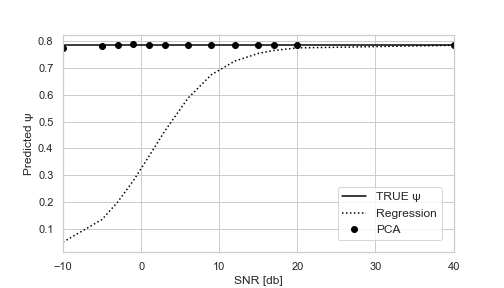
\includegraphics[width=6cm]{performance_comparison.png}
        \caption{コンピュータシミュレーションの結果(位相角は1/4πに固定)}
        \label{simulation}
    \end{center}
\end{figure}

\subsection{有線実験}
シミュレーションでの結果が実機でも成り立つのかを確認するために、図\ref{experiment}のような実験環境を有線で作成し、検証を行なった。
図\ref{lms}, \ref{pca}はそれぞれ最小二乗推定量とPCA推定量の推定結果を表しているが、最小二乗推定量がノイズの影響を強く受けるのに対し、PCA推定量ではノイズの影響をほとんど受けていない様子が確認できる。

\begin{figure}[htbp]
    \begin{center}
        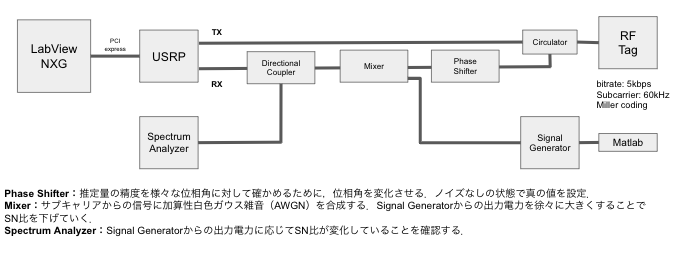
\includegraphics[width=6cm]{experiment.png}
        \caption{有線実験のイメージ図}
        \label{experiment}
    \end{center}
\end{figure}

\begin{figure}[htbp]
    \begin{center}
        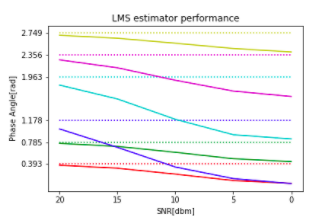
\includegraphics[width=6cm]{lms_performance.png}
        \caption{有線実験の結果}
        \label{lms}
    \end{center}
\end{figure}

\begin{figure}[htbp]
    \begin{center}
        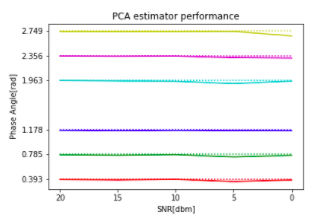
\includegraphics[width=6cm]{pca_performance.png}
        \caption{有線実験の結果}
        \label{pca}
    \end{center}
\end{figure}

\section{考察}
これまでバックスキャッタ信号の位相角推定問題には線形回帰が用いるのが一般的だったが、これはSN比が大きい状況では推定誤差が大きくなる。
しかし、最小二乗推定量はその分母にノイズの分散を含むため、ノイズが大きい環境では推定精度が悪化する。
それに対し、本研究で示したように主成分分析を用いた解法ではノイズの項を一切含まないためSN比が悪い状況でも正確に位相角を推定できる。
したがって、バックスキャッタ信号の位相角推定を行う際には本研究の提案する主成分分析に基づいた手法が有効である。

\bibliographystyle{junsrt}
\bibliography{resume}

\end{document}
% end of file
